\newpage
\section{Parallel Algorithm}

To describe a parallel algorithm
\begin{itemize}
    \item Parallel Random Access Machine (PRAM)
    \item Work-Depth (WD)
\end{itemize}

\subsection{PRAM}
A PRAM employs $p$ synchronous processors, all having unit time access to a shared memory. Each processor has a local memory. At each time unit, a processor can read/write/do some computation with respect to its local memory. 

\begin{figure}[!htb]
    \centering
    
\includegraphics[width=0.309\textwidth]{ADS14/PRAM}
    \caption{PRAM}
\end{figure}

e.g.
\begin{lstlisting}[language={c++}]
for P_i, 1 <=i<=n pardo
    A(i):=B(i)
\end{lstlisting}

\subsubsection{To resolve access conflicts}
\begin{itemize}
    \item Exclusive-Read Exclusive-Write (EREW)
    \item Concurrent-Read Exclusive-Write (CREW)
    \item Concurrent-Read Concurrent-Write (CRCW)
    \begin{itemize}
        \item Arbitrary rule
        \item Priority rule ($P$ with the smallest number)
        \item Common rule (if all the processors are trying to write the same value)
    \end{itemize}   
\end{itemize}

\subsection{The summation problem}
Input:  $A(1), A(2), \dots, A(n)$

Output: $A(1) + A(2) + \dots +A(n)$

\begin{figure}[!htb]
    \centering
    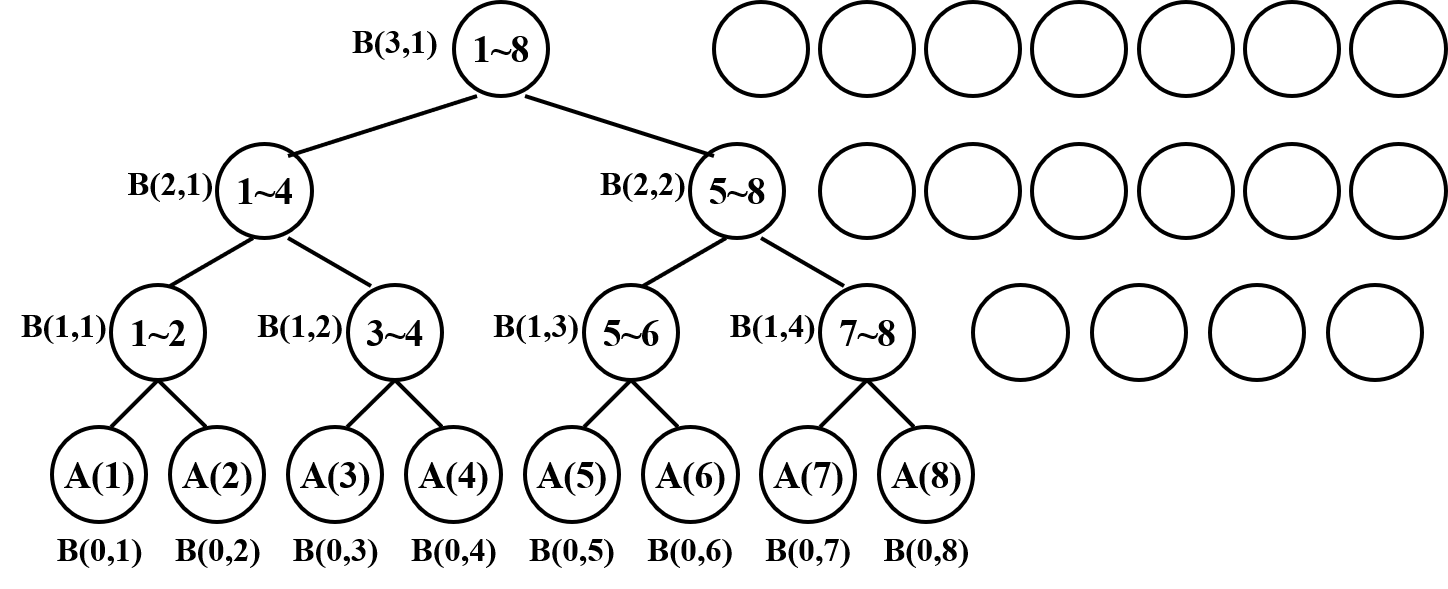
\includegraphics[width=0.42\textwidth]{ADS14/The summation problem}
    \caption{The summation problem $B(h,i)=B(h-1, 2i-1)+B(h-1, 2i)$}
\end{figure}

\subsubsection{PRAM model}
\begin{lstlisting}[language={c++}]
for(P_i, 1<=i<=n)pardo{
    B(0, i):=A(i);
    for(h=1 to logn)do{
        if(i<=n/(2^h))
            B(h, i):=B(h-1, 2i-1)+B(h-1, 2i);
        else stay idle
    }
}
\end{lstlisting}
$T(n)=\log n+2$

\subsubsection{Work-Depth (WD) Presentation}
\begin{lstlisting}[language={c++}]
for(P_i, 1<=i<=n)pardo
    B(0, i):=A(i);
for(h=1 to logn)
    for(P_i, 1<=i<=n/(2^h))pardo{
        B(h, i):=B(h-1, 2i-1)+B(h-1, 2i);
    }
\end{lstlisting}


\subsection{Measuring the performance}
\begin{itemize}
    \item Work load – total number of operations: $W(n)$
    \item Worst-case running time: $T(n)$
\end{itemize}

All asymptotically equivalent:
\begin{enumerate}\small
    \item  $W(n)$ operations and $T(n)$ time
    \item $P(n) = \frac{W(n)}{T(n)}$ processors and $T(n)$ time (on a PRAM)
    \item $\frac{W(n)}{p}$ time using any number of $p \le \frac{W(n)}{T(n)}$ processors (on a PRAM)
    \item $\frac{W(n)}{p} + T(n)$ time using any number of $p$ processors (on a PRAM)
\end{enumerate}

\subsection{Prefix-Sums}
Input:  $A(1), A(2), \dots, A(n)$

Output: $\displaystyle \sum_{i=1}^1A(i), \sum_{i=1}^2A(i), \dots, \sum_{i=1}^nA(i)$

Technique: Balanced Binary Trees

\begin{figure}[!htb]
    \centering
    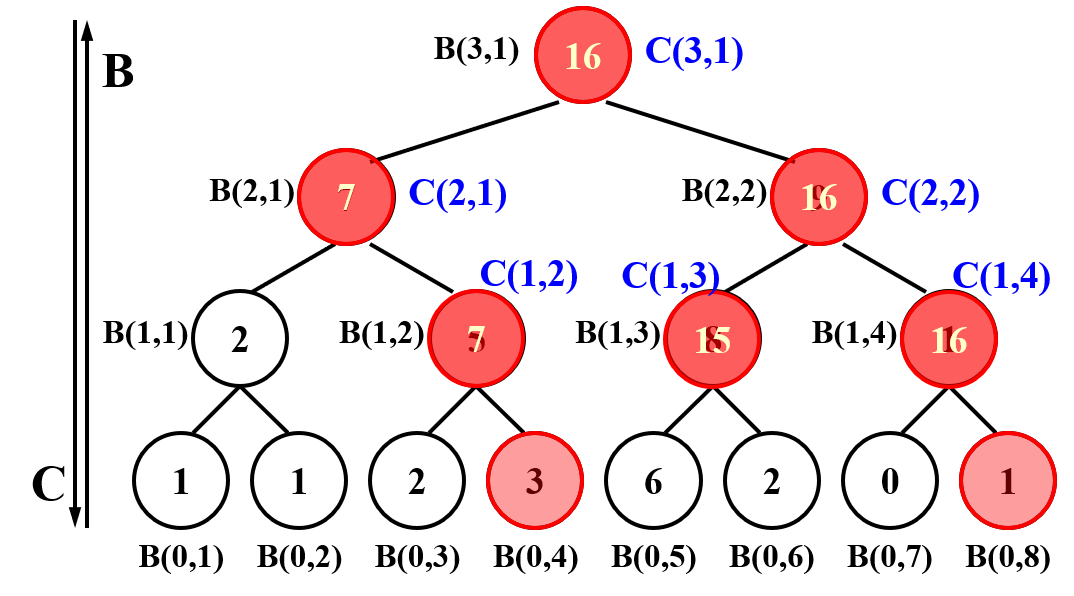
\includegraphics[width=0.42\textwidth]{ADS14/Prefix-Sums}
    \caption{Prefix-Sums}
\end{figure}

\begin{align*}
    C(h,i)=\sum_{k=1}^\alpha A(k)
\end{align*}
where $(0, \alpha)$ is the rightmost descendant leaf of node $(h,i)$. 
\begin{lstlisting}[language={c++}]
if(i==1)C(h,i):=B(h,i);
else if(i%2==0)C(h,i):=C(h+1,i/2);
else if(i%2==1)C(h,i):=C(h+1,(i-1)/2)+B(h,i);
\end{lstlisting}

\subsection{Merging}
Merge two non-decreasing arrays $A(1), A(2), \dots, A(n)$ and $B(1), B(2), \dots, B(m)$ into another non-decreasing array $C(1), C(2), \dots, C(n+m)$. 

Technique: Partitioning

To simplify, assume:
\begin{enumerate}
    \item  the elements of A and B are pairwise distinct
    \item $n = m$
    \item both $\log n$ and $n/\log n$ are integers
\end{enumerate}

\subsubsection{Parallel Ranking}
The ranking problem, denoted RANK(A,B) is to compute: 
\begin{enumerate}
    \item $RANK( i, B)$ for every $1 \le i \le n$, and
    \item $RANK( i, A)$ for every $1 \le i \le n$
\end{enumerate}
\begin{align*}
    \begin{array}{ll}
        RANK( j, A) = i& \text{ if }A(i) < B(j) < A(i + 1), i\in [1, n)\\
        RANK( j, A) = 0& \text{ if }B(j) < A(1)\\ 
        RANK( j, A) = n& \text{ if }B(j) > A(n)
    \end{array}
\end{align*}

\begin{claim}
    Given a solution to the ranking problem, the merging problem can be solved in $O(1)$ time and $O(n+m)$ work.
\end{claim}
\begin{lstlisting}[language={c++}]
for(Pi, 1<=i<=n)pardo
    C(i+RANK(i,B)):=A(i)
for(Pi, 1<=i<=n)pardo
    C(i+RANK(i,A)):=B(i)
\end{lstlisting}

\begin{enumerate}
    \item Partitioning: $p=\frac{n}{\log n}$
    \begin{align*}
        \begin{array}{ll}
            A_{Select}( i ) = A( 1+(i-1)\log n )&i \in [1, p]\\
            B_{Select}( i ) = B( 1+(i-1)\log n )&i \in [1, p]
        \end{array}
    \end{align*}
    Compute $RANK$ for each selected element. 

    \begin{figure}[!htb]
        \centering
        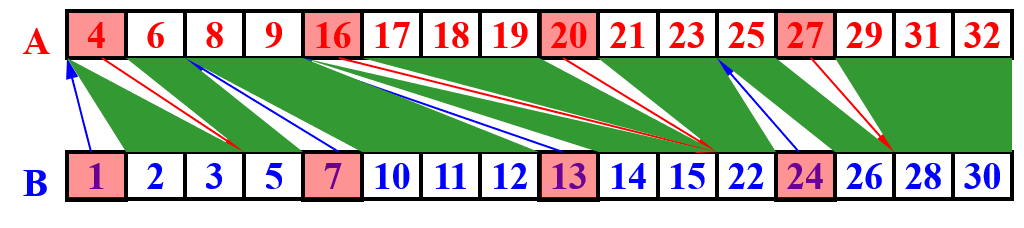
\includegraphics[width=0.42\textwidth]{ADS14/Partitioning}
        \caption{Partitioning}
    \end{figure}
    $T=O(\log n)$, $W=O(p\log n)=O(n)$
    \item Actual Ranking: At most $2p$ smaller sized ($O(\log n)$) problems.

    $T=O(\log n)$, $W=O(p\log n)=O(n)$
\end{enumerate}
$T=O(\log n)$, $W=O(n)$

\subsection{Maximum Finding}
Replace ``$+$'' by ``$\max$'' in the summation algorithm. 

\subsubsection{Compare all pairs}
\begin{lstlisting}[language={c++}]
for(Pi, 1<=i<=n)pardo
    B(i):=0;
for(i and j, 1<=i,j<=n)pardo
    if((A(i)<A(j))||((A(i)=A(j))&&(i<j)))
        B(i)=1;
    else B(j)=1;
for(Pi, 1<=i<=n)pardo
    if(B(i)==0)A(i) is a maximum in A;
\end{lstlisting}
Using common CRCW to resolve access conflicts. 

$T(n)=O(1)$, $W(n)=O(n^2)$

\subsubsection{A Doubly-logarithmic Paradigm}
Assume that $h = \log \log n$ is an integer ($\displaystyle n=2^{2^h}$).

Partition by $\sqrt{n}$:{\small
\begin{align*}
    \begin{array}[pos]{ll}
        A_1=A(1),\dots,A(\sqrt{n})&\Rightarrow M_1 \sim T(\sqrt{n}), W(\sqrt{n})\\
        A_2=A(\sqrt{n}+1),\dots,A(2\sqrt{n})&\Rightarrow M_2 \sim T(\sqrt{n}), W(\sqrt{n})\\
        &\cdots \\
        A_{\sqrt{n}}=A(n-\sqrt{n}+1),\dots,A(n)&\Rightarrow M_{\sqrt{n}} \sim T(\sqrt{n}), W(\sqrt{n})
    \end{array}\\
    M_1,\dots,M_{\sqrt{n}}\Rightarrow A_{\max}\sim \begin{array}{l}
        T=O(1)\\
        W=O(\sqrt{n}^2)=O(n)
    \end{array}
\end{align*}}
\begin{align*}
    &\left\{\begin{array}{l}
        T(n)\le T(\sqrt{n})+c_1\\
        W(n)\le \sqrt{n}W(\sqrt{n})+c_2 n
    \end{array}\right.
    \Rightarrow&\begin{array}{l}
        T(n)=O(\log \log n)\\
        W(n)=O(n \log \log n)
    \end{array}
\end{align*}

Partition by $h = \log \log n$:{\small
\begin{align*}
    \begin{array}[pos]{ll}
        A_1=A(1),\dots,A(h)&\Rightarrow M_1 \sim  O(h)\\
        A_2=A(h+1),\dots,A(2h)&\Rightarrow M_2 \sim O(h)\\
        &\cdots \\
        A_{n/h}=A(n-h+1),\dots,A(n)&\Rightarrow M_{n/h} \sim O(h)
    \end{array}\\
    M_1,\dots,M_{n/h}\Rightarrow A_{\max}
\end{align*}}
\begin{align*}
    \begin{array}{l}
        T(n)=O(h+\log \log (n/h))=O(\log \log n)\\
        W(n)=O(h(n/h)+(n/h)\log\log(n/h))=O(n)
    \end{array}
\end{align*}

\subsubsection{Random Sampling}
with very high probability, on an Arbitrary CRCW PRAM

\begin{figure}[!htb]
    \centering
    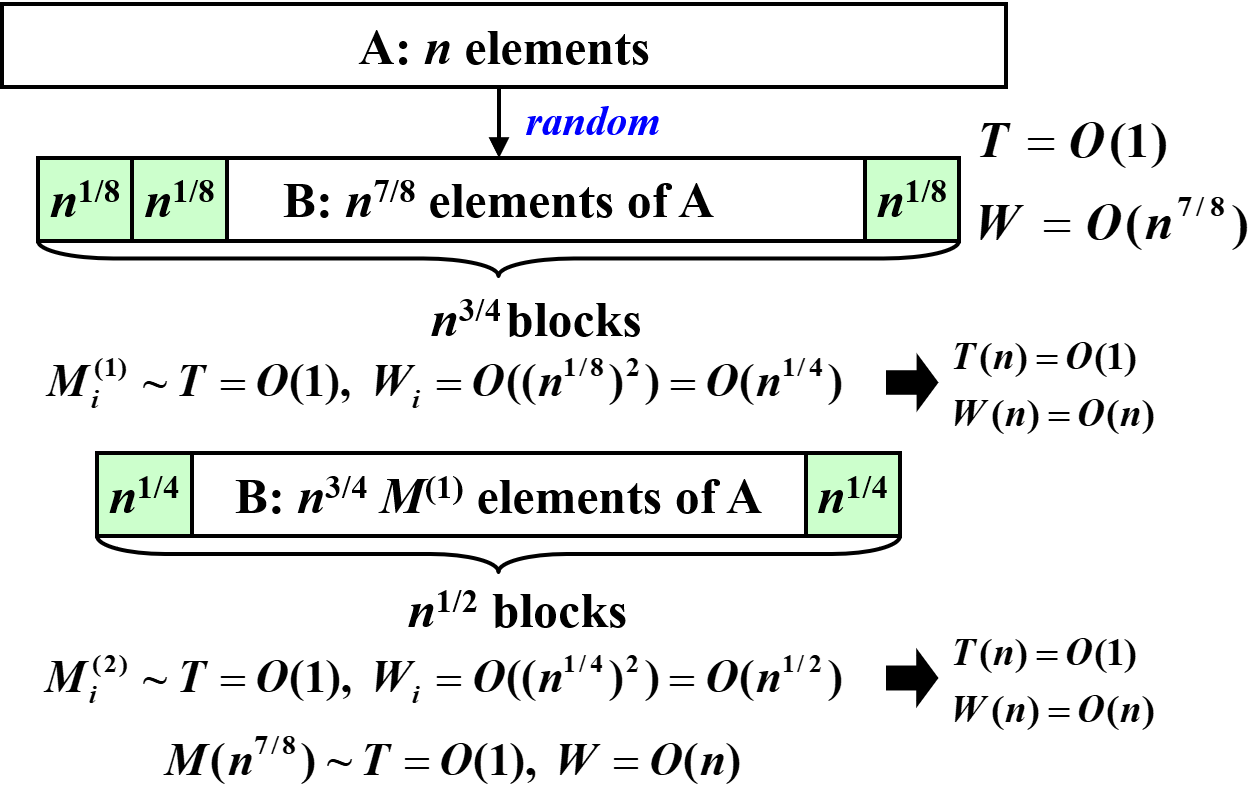
\includegraphics[width=0.42\textwidth]{ADS14/Random Sampling}
    \caption{Random Sampling}
\end{figure}

\begin{theorem}
    The algorithm finds the maximum among $n$ elements.  With very high probability it runs in $O(1)$ time and $O(n)$ work.  The probability of not finishing within this time and work complexity is $O(1/n^c)$ for some positive constant $c$.
\end{theorem}